\chapter{3D Deep Learning}

对于点云来说,直接拉成vector显然是不行的.因为点云本身无序.有一些直接的处理方法:转换成voxel grid(从点云到表面,再重建voxel),或者2D 投影(这属于是越活越回去了).我们想要的network需要对$N!$种不同的点云顺序具有不变性.

一种想法:排序赋予序关系如何?

我们用Permutation Invariant的函数:Symmetric Function.也就是
\begin{equation}
    f(x_1, x_2, \cdots, x_n) \equiv f(x_{\pi_1}, x_{\pi_2}, \cdots, x_{\pi_n}), \forall x \in \mathbb R^N
\end{equation}

实际上,这样的函数随处可见.比如均值,极值等.文献\cite{PointNet} 、PointNet.\footnote{王老师:"虽然我不在这个组里,但PointNet这篇论文的诞生我也是亲眼目睹过的,ICCV的投稿截止在11月,9月底大家还不知道投什么,于是有人说要不试试PointNet吧.写到最后只有两个周调参了,还是打不过voxel,于是加了T-transform.我们这里不讲,因为现在几乎没有用这个的了".(笑)}

\begin{figure}[htbp]
    \centering
    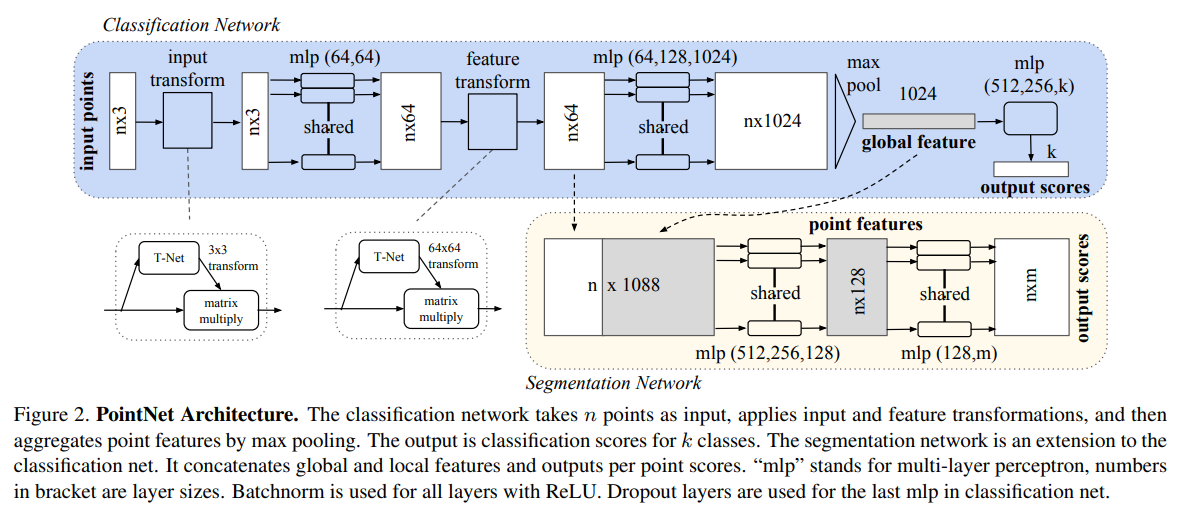
\includegraphics[scale=0.6]{figures/PointNet.png}
    \caption{PointNet的结构图}
\end{figure}

做segmentation:将每个点自身的特征(local)和global feature结合,过MLP就能进行分类.

诸多挑战:Resolution,Occlusion,Noise,Registration.

PointNet对于Resolution和Noise比较robust.在ModelNet40上,去掉50\%的数据,Furthest的准确率只下降了2\%.
能够如此稳定的关键在于max函数,在连续取样时,一些点的丢失可以用周围的点来弥补.而且如果pointnet只有1024个feature,
那么它最多也只会选取1024个点,可能去掉的点根本就没有用到.

\textbf{\\PointNet的不足}

一步直接maxpooling,没有local context.
但是PointNet仍是目前不追求过高性能时对point cloud处理的首选方法.

因为这个不足,有了PointNet++.
即设定一定的范围,将某个点及其周围的点过MLP,再maxpooling.等同于在image里进行conv.当然,求neighbour可能比较花时间.
另外,所有的neighbour都通过了同样的MLP,毕竟在点云里也无法和图像一样,使用卷积核直接提取局部特征.

\begin{figure}[htbp]
    \centering
    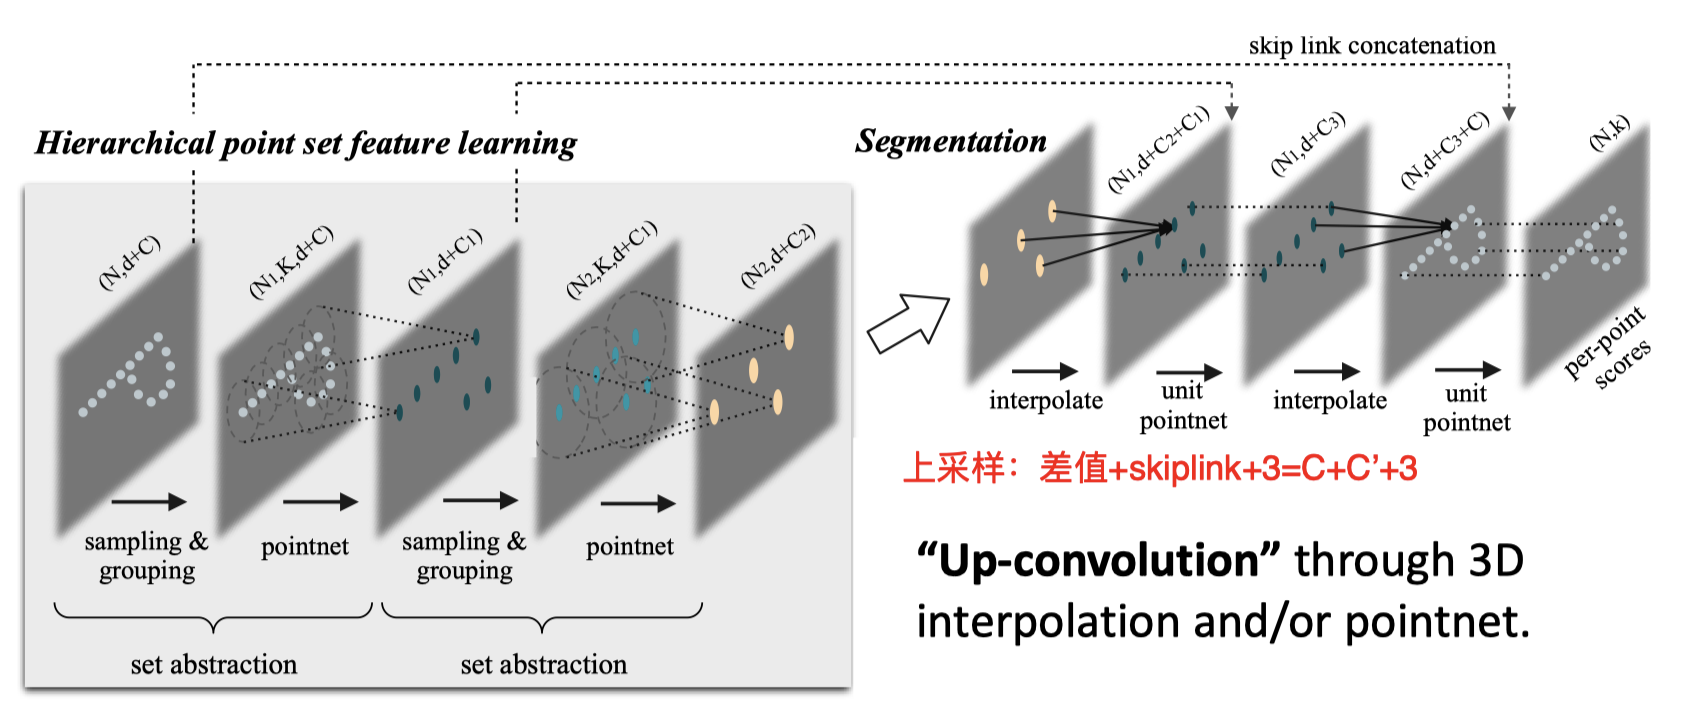
\includegraphics[scale=0.2]{figures/pointnet++.png}
    \caption{PointNet++ Pipeline}
\end{figure}

\textbf{\\PointNet++怎么进行下采样?} 2d中是pooling,而pointnet则进行grouping

\textbf{\\PointNet++怎么进行上采样?}
使用 Skip-Link,将下采样产生的点输入回来.

上采样时候添加的点没有feature, 所以进行interpolate,
新的点选择与它最近的三个点,按照距离反比为权插值获得特征, 这里skip-link是必要的, 否则无法获得点的具体位置.

\section{Sparse Conv}

3D:voxel Net$\rightarrow$sparse conv,屏蔽没有值的voxel,Hash有值的坐标,从NVIDIA,cuda的层次写起.

\begin{figure}[H]
    \centering
    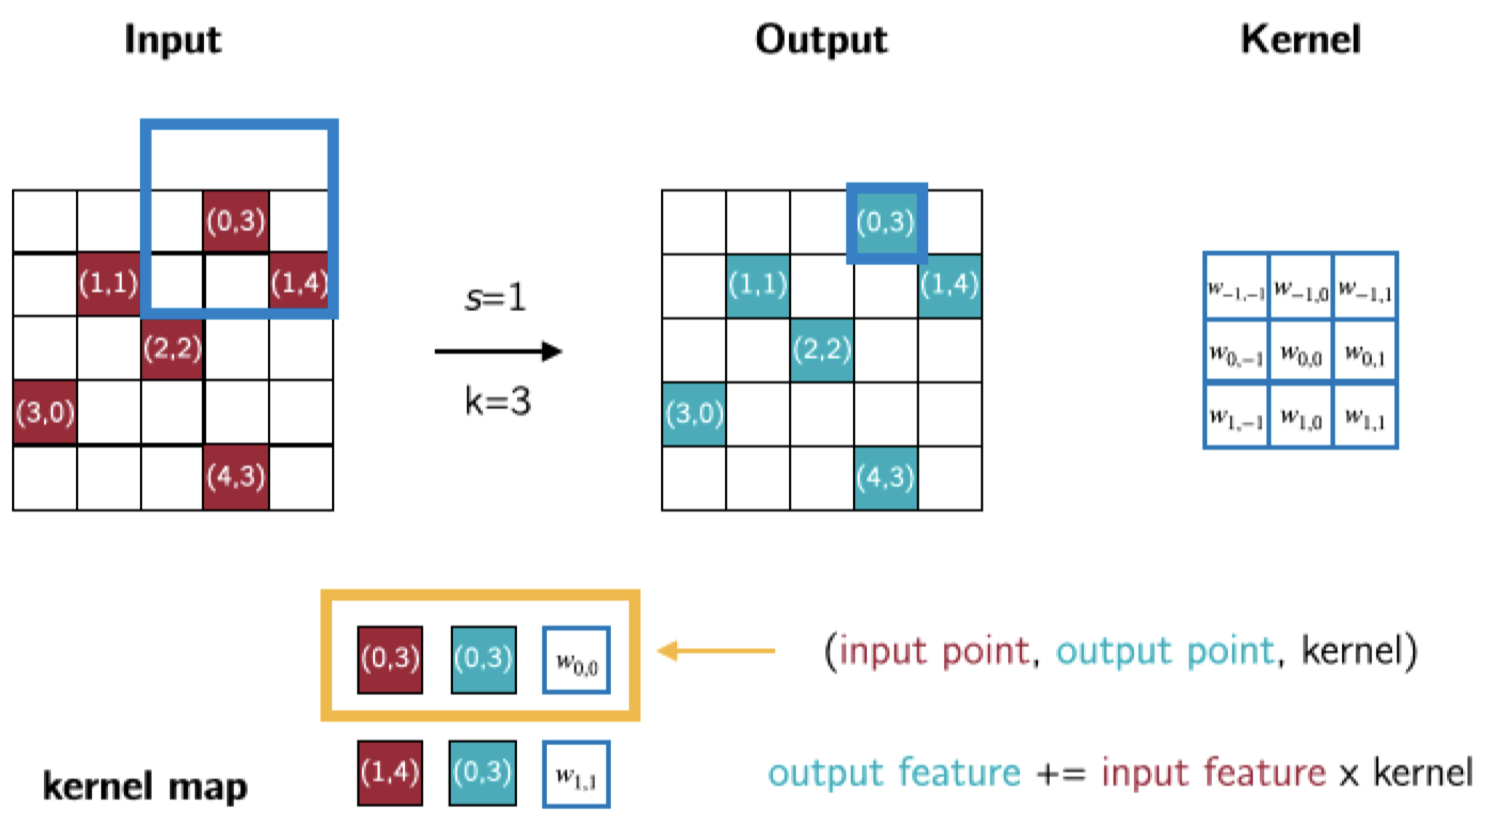
\includegraphics[scale=0.2]{figures/sparsenet.png}
    \caption{Sparse Conv}
    \label{fig:sparsenet}
\end{figure}

结合图示\ref{fig:sparsenet}来理解稀疏卷积的过程:

\begin{enumerate}
\item 输入特征图:图中的红色方块表示非零值的位置,比如在输入特征图中,位置 (0,3)、(1,1)等具有非零值.
\item 卷积核:一个 3$\times$3 的卷积核,包含权重参数 $w_{-1,-1}$ 等.
\item 输出特征图:稀疏卷积的输出特征图.只有当卷积核的中心对准输入特征图的非零值时,才会计算输出值.
\item 稀疏卷积过程:当卷积核的中心对准输入特征图的 (0,3) 位置时,计算对应的输出值.
例如,卷积核中心对准 (0,3) 时,只有卷积核的中心权重 ($w_{0,0}$) 参与计算,输出值为:\[ \text{output}(0,3) = \text{input}(0,3) \times w_{0,0} \]
当卷积核中心对准 (1,4) 位置时,计算对应的输出值,输出值为:\[ \text{output}(1,4) = \text{input}(1,4) \times w_{1,1} \]
\item 通过这种方式,稀疏卷积仅计算非零值对应的输出,从而减少了大量的计算和内存开销.
\end{enumerate}

Sparse conv:kernel 是空间各向异性(spatial anisotropic)的.因此它的acc能够达到惊人的70\%以上,
而point cloud无论如何添加特性,最多也在64\%左右.而且因为可被标签,使用更加方便.但是它的分辨率受限.

\textbf{\\Sparse Conv Pros and Cons?}

Sparse Conv优点:
\begin{enumerate}
    \item 比dense conv更高效,稀疏卷积只对非零值进行计算,跳过零值,从而显著减少了计算量和内存使用,提高了计算效率.
    \item 支持索引的网格, 稀疏卷积仍然在规则的网格上操作,这意味着可以利用现有的索引机制来高效地访问数据.
    \item 与2D Conv具有类似的表达能力
    \item 与2D Conv具有类似的平移等变性
\end{enumerate}

Sparse Conv缺点:
\begin{enumerate}
    \item 离散化误差, 由于稀疏卷积只对非零值进行计算,可能会导致离散化误差.这种误差源于对数据的稀疏表示,可能会影响卷积操作的精确性.
\end{enumerate}

\textbf{\\Sparse Conv vs. Point Cloud Networks?}

Sparse Conv:
\begin{enumerate}
    \item 优点:核是空间各向异性的
    \item 优点:更高效的索引和近邻查询
    \item 优点:适用于大规模场景
    \item 缺点:分辨率有限
\end{enumerate}

Point Cloud Nets:
\begin{enumerate}
    \item 优点:分辨率高
    \item 优点:鲁棒性强
    \item 缺点:表现稍差一些
    \item 缺点:执行 Farthest Point Sampling 和 Ball Query 等操作较慢
\end{enumerate}

\section{PointNet++ V.S. Conv}

PointNet++相当于卷积网络的先做 $1\times 1$ conv 然后 $n\times n$ MaxPooling,都是变少了点的数目,但是每一个点的特征变多了

区别在于:PointNet++对于一个局域部分,不同的点是各向同性的,但是卷积网络对于一个局域是不同的,因为一个卷积核不同位置的权不一样.

具体表现在:如果把一个邻域内的点更换位置,那么PointNet++的结果不变,但是卷积网络的结果会变.

这是由于两个原因:
\begin{enumerate}
    \item 卷积网络的卷积核是 $3\times 3$ 的,而PointNet++的MLP是全局的,相当于$1\times 1$的CONV,而$1\times 1$的CONV很容易想到是各向同性的,
    如果把一个邻域内的点更换位置,那么每个点的MLP结果不变.
    \item 卷积网络的MaxPooling不是全局的,而PointNet++的MaxPooling是全局的,因此如果把一个邻域内的点更换位置,
    那么卷积网络的结果会变,而PointNet++的结果不变,因为怎么变换位置都是取最大值.
\end{enumerate}

PointNet:$C\times C^\prime$ params

ConvNet: $3\times 3\times C\times C^\prime$ params

\section{设计一个二维PointNet}

如何设计一个二维的pointnet呢?

我们可以将图片看作二维的点云, 对于每一个像素 $x_i$, 将其颜色或者透明度等信息看作是 $x_i$ 的三维坐标,然后使用pointnet的方法进行处理

具体来讲, 图片维度为 $H\times W\times C$, 那么我们可以将其看作 $H\times W$ 个点, 每个点的特征是 $C$ 维的, 
每一个像素通过相同的MLP映射到 $C^\prime$ 维, 然后进行maxpooling, 最终得到 $C^\prime$ 维的全局特征.